% chercher des documents LaTeX dans styles, corps et bib
\makeatletter\def\input@path{{styles/}{corps/}}\makeatother

% Utiliser le style rapport.cls
\documentclass{rapport}

\title{Modélisation et simulation d'un environnement sous-marin pour Forssea Robotics}
\author{Quentin \textsc{Brateau} \\ \texttt{quentin.brateau@ensta-bretagne.org} \\[10mm]{\small Encadrant école \\Luc \textsc{Jaulin} \\\texttt{luc.jaulin@ensta-bretagne.fr}} \\[5mm]{\small Encadrant entreprise \\Alaa \textsc{El Jawad} \\\texttt{alaa@forssea-robotics.fr}}}
\date{\today}
\doctype{Rapport de PFE}
\promo{FISE 2021}
\etablissement{\textsc{Ensta} Bretagne\\2, rue François Verny\\
  29806 \textsc{Brest} cedex\\\textsc{France}\\Tel +33 (0)2 98 34 88 00\\ \url{www.ensta-bretagne.fr}}
\logoEcole{
\includegraphics[height=4.2cm]{logo_ENSTA_Bretagne_Vertical_CMJN}}

\hypersetup{
  pdftitle={Rapport de PFE},
  pdfauthor={Quentin Brateau},
  pdfkeywords={guide, rapport de projet},
  bookmarksnumbered,
  pdfstartview={FitH},
  citecolor=blue,
  breaklinks=true
}

% creer le glossaire
\makeglossaries
% creer l'index
\makeindex

\begin{document}
	% Début du préambule
	\frontmatter
	% inclure la liste des acronymes
	\newglossaryentry{ENSTAB}{type=glo,
	text={\textsc{ENSTA} Bretagne},
	name={\textsc{ENSTA} Bretagne},
	description={Ecole Nationale Supérieure de Techniques Avancées Bretagne}}

\newglossaryentry{ROV}{type=glo,
	text={\textsc{ROV}},
	name={\textsc{ROV}},
	description={Remotely Operated Vehicles, véhicule sous-marin téléguidé}}

\newglossaryentry{Argos}{type=glo,
	text={\textsc{Argos}},
	name={\textsc{Argos}},
	description={\gls{ROV} commercialisé par Forssea Robotics}}

\newglossaryentry{Atoll}{type=glo,
	text={\textsc{Atoll}},
	name={\textsc{Atoll}},
	description={\gls{ROV} commercialisé par Forssea Robotics}}

\newglossaryentry{Navcam}{type=glo,
	text={\textsc{Navcam}},
	name={\textsc{Navcam}},
	description={camera de navigation réalisant un traitement temps-réel basé sur des algorithmes d'intelligence artificielle}}

\newglossaryentry{Obscam}{type=glo,
	text={\textsc{Obscam}},
	name={\textsc{Obscam}},
	description={camera d'observation}}

\newglossaryentry{frameLBL}{type=glo,
	text={\textsc{Frame lbl}},
	name={\textsc{Frame lbl}},
	description={Cadre portant des balise Long Baseline permettant la localisation sous-marine}}

\newglossaryentry{Gazebo}{type=glo,
	text={\textsc{Gazebo}},
	name={\textsc{Gazebo}},
	description={Logiciel de simulation multi-physique dédié à la robotique : \url{http://gazebosim.org/}}}

\newglossaryentry{ROS}{type=glo,
	text={\textsc{ROS}},
	name={\textsc{ROS}},
	description={Middleware dédié à la robotique : \url{https://www.ros.org/}}}

\newglossaryentry{Plugin}{type=glo,
	text={\textsc{Plugin}},
	name={\textsc{Plugin}},
	description={Module d'extension permettant d'ajouter des fonctionnalités à un logiciel}}

\newglossaryentry{Cpp}{type=glo,
	text={\textsc{C++}},
	name={\textsc{C++}},
	description={Language de programmation}}

\newglossaryentry{GSL}{type=glo,
	text={\textsc{GSL}},
	name={\textsc{GSL}},
	description={GNU Scientific Library, une librairie \gls{Cpp} permettant de résoudre des problèmes mathématiques}}
	% creer le titre ici
	\maketitle

	% chargement du fichier abstract.tex
	
\section*{R�sum�}
  Dans le cadre de ses fonctions, l'ing�nieur se doit de ma�triser les
  techniques de base de r�daction de documents.

  Le pr�sent guide fournit les premiers �l�ments visant � la r�daction d'un
  rapport de projet. Il est destin� aux �l�ves effectuant un projet dans le
  cadre de leur scolarit� � l'\gls{enstab}.  Sont pr�sent�s, de fa�on
  synth�tique, les bases sur la nature et la structure du rapport, ses r�gles
  de composition et de typographie.

\section*{Mots cl�s}
Rapport de projet, m�moire, r�daction.

\selectlanguage{english}
\section*{Abstract}
  In the context of their profession, engineers have to master basic
  techniques for writing documents.
  
  This guide provides the fundamental elements for writing a project
  report. It is intended for students undertaking projects during their
  studies at \gls{enstab} and it gives an overview of the basics in
  relation to the nature and components of a report, with formatting
  guidelines and typographic rules.
  
\section*{Keywords}
Project report, memoir, writing.

\selectlanguage{french}

\section*{Remerciements}

Je remercie Nathalie Debese, Amandine Nicolle, Olivier Reynet et H�l�ne Thomas
pour leur travail de relecture.


%%% Local Variables: 
%%% mode: latex
%%% TeX-master: "../guide"
%%% End: 


	\clearpage

	% table des matieres
	\tableofcontents

	\clearpage

	% Partie principale
	\mainmatter

	\chapter{Introduction}
	
	\section{Forssea Robotics}

		Forssea Robotics est une jeune entreprise innovante en matière de robotique sous-marine. Elle propose des solutions industrielles à l'exploration de ce milieu particulièrement hostile à l'homme. Ils excellent principalement dans les quatre domaines suivants robotique autonome, ingéniérie des \gls{ROV}s, vision sous-marine et intelligence artificielle, ce qui leur vaut de travailler aux côtés de nombreux partenaires, comme le groupe Total, Thales, iXblue, DeepOcean, et bien d'autres, mais aussi des centre de recherches comme l'\gls{ENSTAB}.

	\section{Présentation du projet de fin d'études}

		\subsection{Sujet}
    Dans les phases de développements des robots, Forssea Robotics doit faire face à de nombreuses problématiques, dont celle de tester les algorithmes impémentés sur les \gls{ROV}s. Pour cela l'entreprise réalise régulièrement des tests et conditions réelles, mais ce sont des essais coûteux et qui prennent beaucoup de temps à plannifier et à organiser. Afin de réduire le nombre d'essais nécéssaires, il serait préférable de développer un moyen de test rapide et fiable des robots dans leur environnement. Cela permettrait à la fois d'augmenter les performances des robots et de diminuer les coûts et les temps de développements.

\subsection{Objectifs}
    L'objectif de ce stage est de construire un environnement de simulation sous-marin pour Forssea Robotics. Il devra permettre de simuler au mieux le comportement des robots dans leur milieu, mais aussi de permettre de tester leurs algorithmes de navigations autonomes. Cet environnement de simulation permet évidemment de tester plus rapidement les implémentations, de construire des situations difficilements trouvables en conditions réelles, mais aussi d'avoir une répétabilité des situations. En outre, il ne se substitue pas à la réalisation de tests en conditions réelles.

    Ce projet de fin d'étude s'inscrit dans le cadre d'un contrat de professionalisation réalisé chez Forssea Robotics. Il m'a permis d'effectuer un premier pas dans le monde industriel tout en finissant ma formation au sein de l'\gls{ENSTAB}. J'ai donc pu avoir un sujet plus complet
	

	\chapter{Conception et analyse du système}

    \section{Introduction}

        La simulation de milieux marins est quelque chose de connu dans le domaine de la robotique, et il en existe aujourd'hui déjà de nombreux~\cite{Manhaes_2016, bingham19toward, MARS, Rock}. Ces simulateurs proposent tous un modèle de flottabilité pour les objets à simuler, ce qui permet de pouvoir définir à la fois des bateaux et des robots sous-marins. Cela permet donc de pouvoir simuler le comportement des \gls{ROV}s dans l'eau. Ils proposent ensuite tous leur lot de spécificités qui permettent d'avoir des éléments supplémentaires dans notre simulation.
        
        \textsc{UUV Simulator}~\cite{Manhaes_2016} est probablement le plus connu d'entre eux. C'est un simulateur de \gls{ROV} comportant un certain nombre d'éléments d'environnements simulés, comme des mondes marins, du courant ou des ombilicaux par exemple. Il propose aussi la description d'un bon nombre de robots sous-marins commercialisés, et la communauté active partage les nouveaux modèles régulièrement.
        
        \textsc{Mars}~\cite{MARS} est un simulateur spécifique à des robot baptisés \textsc{Mars}. Il permet de supporter plusiieurs \gls{ROV}s et peut être commandé par \gls{ROS} ou bien en utilisant des sockets TCP.
        
        \textsc{Rock-Gazebo}~\cite{Rock} est un projet d'intégration de simulateur basé sur le moteur physique \gls{Gazebo} et sur le framework\footnote{Infrastructure logicielle facilitant le développement logiciel} \textsc{Robot Construction Kit}.
        
        Le simulateur \textsc{VRX}~\cite{bingham19toward} est un projet open-source de robotique marine dont un simulateur a été implémenté sur la base de \gls{Gazebo}. Il propose un ensemble d'environnement, de modèles et de plugin permettant la simulation de missions de vaisseaux de surface, avec notamment la possibilité de prendre en compte la présence de vagues et de vent à la surface.

        Ces simulateurs proposent tous des spécificités différentes et intéressantes. Cependant, notre application de simulation de \gls{ROV}s pour \textsc{Forssea Robotics} est assez contrainte. En effet, l'existance de composants spécifiques, comme la simulation du \gls{Latch} ainsi que la \gls{frameLBL} rendent l'adaptation de simulateurs déjà existants trop difficile. C'est pourquoi il est nécéssaire de réaliser notre propre simulateur.

    \section{Spécifications fonctionnelles}
        \label{sec:spec_fonc}

        Le système à concevoir doit permettre de simuler \gls{ROV}s de la société \textsc{Forssea Robotics} dans un environnement sous-marin. Le simulateur doit respecter un certain nombre de spécifications fonctionnelles qui délimitent les exigences requises par le système. La \textsc{Figure}~\ref{figure:pieuvre} complétée par la \textsc{Table}~\ref{table:specs} présentent les exigences du système.

        \begin{figure}[!htb]
            \centering
            \begin{tikzpicture}[scale=0.7, every node/.style={ellipse, align=center, scale=0.7}]
                \node[draw,minimum height=40pt, minimum width=100pt, fill=Lavender!80!pink!100] (S) at (0, 0) {Simulateur};
                \node[draw,minimum height=40pt, minimum width=100pt, fill=cyan!60!pink!70] (C0) at (25:5.5cm) {Robot};
                \node[draw,minimum height=40pt, minimum width=100pt, fill=cyan!60!pink!70] (C1) at (155:5.5cm) {Environnement};
                \node[draw,minimum height=40pt, minimum width=100pt, fill=cyan!60!pink!70] (C2) at (205:5.5cm) {Communication};
                \node[draw,minimum height=40pt, minimum width=100pt, fill=cyan!60!pink!70] (C3) at (335:5.5cm) {Interface};
                
                \draw[blue!75, line width=0.8mm] (C0) -- (S) node[midway, fill=white]{FP1};
                \draw[blue!75, line width=0.8mm] (C1) -- (S) node[midway, fill=white]{FP2};
                \draw[orange!80, line width=0.8mm] (C2) -- (S) node[midway, fill=white]{FC1};
                \draw[orange!80, line width=0.8mm] (C3) -- (S) node[midway, fill=white]{FC2};
            \end{tikzpicture}
            \caption{Diagramme pieuvre du simulateur}
            \label{figure:pieuvre}
        \end{figure}

        \begin{table}[!htb]
            \centering
            \begin{adjustbox}{max width=\textwidth}
                \begin{tabularx}{\textwidth}{|lX|}
                    \hline
                    \cellcolor{gray!25}\textbf{id} & \cellcolor{gray!25} \textbf{Fonction} \\
                    \hline \hline
                    \cellcolor{blue!30}\textbf{FP1}&\cellcolor{blue!25} Le système doit avoir un comportement proche du robot réel. \\
                    \hline
                    \cellcolor{gray!10}FP1.1& Le système doit avoir des dimensions semblables au robot réel. \\
                    \hline
                    \cellcolor{gray!10}FP1.2& Le système doit avoir des masses et des inerties semblables au robot réel. \\
                    \hline
                    \cellcolor{gray!10}FP1.3& Le système doit avoir les mêmes degrès de liberté que le robot réel. \\
                    \hline
                    \cellcolor{gray!10}FP1.5& Le système doit avoir les mêmes actionneurs que le robot réel. \\
                    \hline
                    \cellcolor{gray!10}FP1.4& Le système doit avoir les mêmes capteurs que le robot réel. \\
            
                    \hline \hline
            
                    \cellcolor{blue!30}\textbf{FP2}&\cellcolor{blue!25} Le système doit simuler l'environnement du robot \\
                    \hline
                    \cellcolor{gray!10}FP2.1& Le système doit simuler l'environnement sous-marin. \\
                    \hline
                    \cellcolor{gray!10}FP2.2& Le système doit simuler la présence de courants marins. \\
                    \hline
                    \cellcolor{gray!10}FP2.2& Le système doit simuler les ombilicaux reliant le \gls{ROV} au bateau. \\
                    \hline
            
                    \hline \hline
            
                    \cellcolor{orange!40}\textbf{FC1} &\cellcolor{orange!30} Le système doit communiquer son état à l'utilisateur. \\
                    \hline
                    \cellcolor{gray!10}FC1.1& Le système doit communiquer l'état du robot à l'utilisateur. \\
                    \hline
                    \cellcolor{gray!10}FC1.2& Le système doit communiquer l'état de l'environnement à l'utilisateur.\\
                    \hline
            
                    \hline \hline
            
                    \cellcolor{orange!40}\textbf{FC2}&\cellcolor{orange!30} Le système doit être interfaceable avec le reste de l'implémentation logicielle. \\
                    \hline
                    \cellcolor{gray!10}FC2.1& Le système doit pouvoir évoluer dans un monde vide. \\
                    \hline
                    \cellcolor{gray!10}FC2.2& Le système doit pouvoir évoluer dans une vigne ayant une largeur paramétrable. \\
                    \hline
                    \cellcolor{gray!10}FC2.3& Le système doit pouvoir entrer en collision avec les objets solides de l'environnement de simulation. \\
                    \hline
                \end{tabularx}
            \end{adjustbox}
            \caption{Spécifications fonctionnelles du simulateur}
            \label{table:specs}
        \end{table}    

    \section{Spécifications techniques}

        Pour remplir les différentes spécifications fonctionnelles présentées dans la \textsc{Section}~\ref{sec:spec_fonc}, nous allons définir un certain nombre de spécifications techniques. Ces dernières vont proposer les outils et les différents critères permettant de remplir les exigences attendues.

        \subsection{Logiciel de simulation}

            L'étude de l'existant nous aura au moins permis de se rendre compte que \gls{Gazebo}~\cite{Koenig-gazebo} est largement utilisé dans le domaine de la simulation sous-marine, mais aussi plus largement dans la simulation robotique. \gls{Gazebo} est un logiciel de simulation multi-physique open-source\footnote{Code communautaire ouvert libre de redistribution et d'accès}. Il est aujourd'hui développé par la communauté \gls{OpenRobotics}. Il présente l'avantage de pouvoir communiquer avec \gls{ROS}, ce qui est une exigence importante de notre simulateur, car il doit permettre de tester l'implémentation logicielle des robots. La description des robots se fait en utilisant le language \gls{SDF}\footnote{\url{http://sdformat.org/}}, et il est possible de décrire le comportement complexe d'un composant en implémentant un \gls{Plugin}.

            L'utilisation de ce logiciel nous permet donc de remplir la fonction principale \textbf{FP1}, dans la mesure où il est possible de décrire tout les composants des \gls{ROV}s avec les trois couches visuelles, de collision et d'inertie, mais aussi les capteurs et les actionneurs dans l'environnement de simulation de \gls{Gazebo}. Il est aussi possible de décrire le comportement de l'environnement du robot dans ce simulateur, ce qui permet de remplir la fonction principale \textbf{FP2}.

        \subsection{Ignition Libraries}

            Ignition Libraries\footnote{\url{https://ignitionrobotics.org/libs}} est un ensemble de libraries permettant de faciliter le développement robotique. Ces librairies sont mises à disposition par \gls{OpenRobotics}. Deux libraries permettent de remplir la fonction contrainte \textbf{FC1} : \textit{Ignition-Transport} et \textit{Ignition-Msgs}. Ces deux libraries permettent de faire communiquer deux ensemble de codes ensemble grâce à un système de messagerie basée sur l'utilisation de la bilbiothèque \textit{ProtocolBuffer} développée par \textit{Google}\footnote{\url{https://developers.google.com/protocol-buffers}}. Enfin, ce système de communication est utilisé par \gls{ROS} et \gls{Gazebo}. Il présente l'avantage de diviser le code en n\oe uds pouvant communiquer ensemble, mais aussi de pouvoir récupérer l'état du simulateur par la lecture des messages transitants sur le réseau \textit{Ignition-Transport}.

        \subsection{ROS2 Control}

            Le simulateur doit permettre de s'interfacer avec le reste de l'implémentation logicielle, il est nécéssaire de définir une architecture logicielle permettant de communiquer à la fois avec les \gls{ROV}s réels et simulés. \gls{ROS2Control}~\cite{ros_control} est un framework permettant de faire communiquer des contrôleurs et des drivers ensemble. L'avantage est de pouvoir changer en fonctionnement de contôleur de manière consistante, sans temps mort durant lesquels le robot ne serait pas commandé.

            \begin{figure}[!htb]
                \centering
                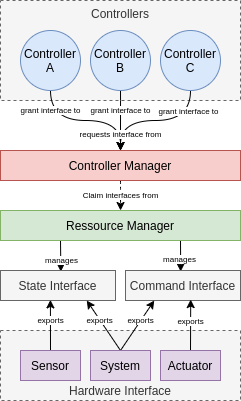
\includegraphics{imgs/ros2_control.pdf}
                \caption{Architecture logicielle avec \gls{ROS2Control}}
                \label{fig:ros2_control}
            \end{figure}

            La \textsc{Figure}~\ref{fig:ros2_control} nous montre l'architecture logicielle de \gls{ROS2Control}. Ce framework va instancier un \gls{ControllerManager} qui va s'occuper de charger les contrôleurs qui seront utilisés dans le robot, des \gls{HardwareInterface} qui sont les interfaces qui vont communiquer avec les composants et un \gls{RessourceManager} qui va faire transiter les données entre les contrôleurs et les composants. L'\gls{HardwareInterface} peut être réelle ou simulées, c'est-à dire qu'elle peut communiquer avec des vrai composants ou des composants simulés. L'idée est de crée une \gls{HardwareInterface} proposant les mêmes interfaces que celle implémentée pour les composants réels. Ainsi on peut utiliser les mêmes algorithmes de contrôle de manière totalement transparente sur les composant réels et les composants simulés.

        \subsection{Architecture Logicielle}

            En rassemblant ce qui a pu être présenté dans cette \textsc{Section}, on peut proposer une architecture logicielle pour ce simulateur présentée sur la \textsc{Figure}~\ref{fig:architecture_logicielle}.
            
            \begin{figure}[!htb]
                \centering
                \includegraphics[]{imgs/architecture_logicielle.pdf}
                \caption{Architecture logicielle du simulateur}
                \label{fig:architecture_logicielle}
            \end{figure}
	
	\chapter{Simulation de l'environnement}
\label{chapitre:environnement}
	
	\section{Introduction}

		La simulation de l'environnement est une partie importante du simulateur car c'est ce qui va définir le comportement des \gls{ROV}s dans leur milieu. Elle doit être très proche des conditions réelles afin d'avoir des résultats exploitables. Il faut donc établir les différents élements de l'environnements qui vont interagir avec les \gls{ROV}s afin de les intégrer dans le simulateur. Il y a principalement le milieu marin qui va ajouter une flottabilité au robots, mais aussi la présence de courants et enfin l'ombilical qui relie les \gls{ROV}s au bateau afin de l'alimenter en énergie mais aussi d'avoir un retour d'informations.

		La simulation de milieux marins est quelque chose de connu dans le domaine de la robotique. Il existe de nombreux simulateurs d'environnements marins et sous-marins~\cite{Manhaes_2016, bingham19toward, MARS, Rock}. Ces simulateurs proposent tous un modèle de flottabilité pour les objets à simuler, ce qui permet de pouvoir définir des bateaux ou bien des robots sous-marins. Cela permet donc de pouvoir simuler le comportement des \gls{ROV}s dans l'eau. Ils proposent ensuite différentes spécificités qui permettent d'avoir des éléments supplémentaires dans notre simulation. \textsc{Mars}~\cite{MARS} est un simulateur spécifique à des robot baptisés \textsc{Mars}. \textsc{Rock-Gazebo}~\cite{Rock} est un projet d'intégration de simulateur basé sur le moteur physique \gls{Gazebo} et sur le framework\footnote{Infrastructure logicielle facilitant le développement logiciel} \textsc{Robot Construction Kit}. Le simulateur \textsc{VRX}~\cite{bingham19toward} est un projet open-source de robotique marine dont un simulateur a été implémenté sur la base de \gls{Gazebo}. Il propose un ensemble d'environnement, de modèles et de plugin permettant la simulation de missions de vaisseaux de surface, avec notamment la possibilité de prendre en compte la présence de vagues et de vent à la surface.

		La \textsc{Table}~\ref{table:elements} présente les différents élements qui peuvent être simulés dans un environnement marin.

		\begin{table}[ht]
			\centering
			\begin{tabular}{|c|c|}
				\hline
				Element & Simulation \\
				\hline
				Vent & \xmark\\
				\hline
				Vagues & \xmark\\
				\hline
				Courant sous-Marin & \cmark \\
				\hline
				Ombilical & \cmark \\
				\hline
			\end{tabular}
			\caption{Elements pris en compte dans l'environnement de simulation}
			\label{table:elements}
		\end{table}

	\section{Simulation d'environnements marins}

		

	\section{Simulation des courants marins}

		Une simulation des courants marins basée sur les équations de Navier-Stokes permet de proposer une approche intéressante à la simulation de courants marins~\cite{Garau2006current}.

	\section{Simulation d'ombilicaux}

		\subsection{Etat de l'art}

\subsection{Formalisme}

\subsection{Initialisation}
    L'initialisation des différents n\oe uds de l'ombilical est une étape importante car les coefficients du modèle comportemental sont reglés pour avoir un comportement cohérent lorsque la position du câble a convergée. Si l'initialisation est aléatoire, le temps du régime transitoire peut être long et la simulation peut ne pas être consistante.

    Pour initialiser l'ombilical, nous allons nous appuyer sur l'équation de la chaînette. Cette équation issue du calcul variationnel représente la forme que prend une corde attachée à ses deux extrémités afin de limiter son énergie. La \textsc{Figure}~\ref{fig:chainette} représente un tracé de cette équation.

    \begin{figure}[!htb]
        \centering
        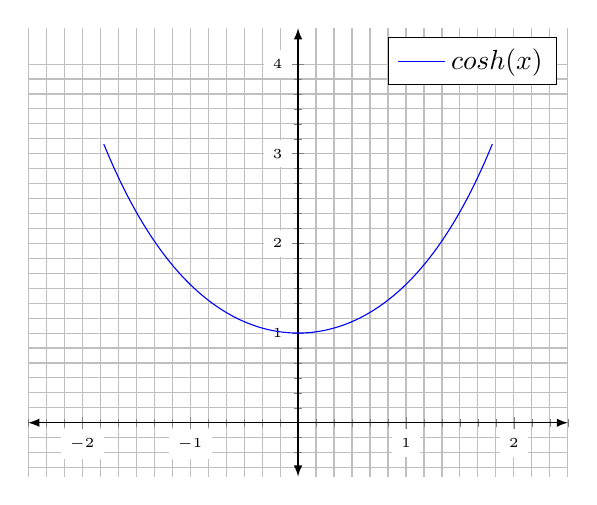
\begin{tikzpicture}
            \begin{axis}[
                    xmin=-2,   xmax=2,
                    ymin=-0.1,   ymax=3.9,
                    grid=both,
                    axis lines=middle,
                    minor tick num=5,
                    enlargelimits={abs=0.5},
                    axis line style={latex-latex},
                    ticklabel style={font=\tiny,fill=white},
                    xlabel style={at={(ticklabel* cs:1)},anchor=north west},
                    ylabel style={at={(ticklabel* cs:1)},anchor=south west}
                ]
                \addplot [
                    domain=-1.8:1.8, 
                    samples=100, 
                    color=blue,
                    ]
                    {cosh(\x)};
                \addlegendentry{$cosh(x)$}
            \end{axis}
        \end{tikzpicture}
        \caption{Représentation graphique de l'équation de la chaînette}
        \label{fig:chainette}
    \end{figure}
    

\subsection{Implémentation}
    L'implémentation d'un \gls{Plugin} \gls{Gazebo} permet de simuler le comportement de l'ombilical dans l'environnement de simulation. Ce \gls{Plugin} est basé sur l'instanciation d'objets de type \textit{Tether} et \textit{TetherElement}. L'objet \textit{Tether} possède les paramètres de simulation de l'ombilical, tandis que l'objet \textit{TetherElement} représente un tronçon de cet ombilical. Un diagramme de classe est présenté en \textsc{Figure}~\ref{fig:uml_class} et montre les différents attributs et méthodes associées à chaque classe.
    
    La \textit{Tether} utilise une structure de liste doublement chaînée\footnote{structure de données liée qui consiste en un ensemble n\oe uds liés les uns aux autres par des références au n\oe uds voisins.} de \textit{TetherElement}. Chaque \textit{TetherElement} possède alors une référence vers l'élément le précédant et l'élément le suivant, comme le montre la \textsc{Figure}~\label{fig:goubly_linked_list}. La \textit{Tether} ne possède ainsi qu'une référence vers le premier et le dernier n\oe ud de la chaîne, nommés respectivements \textit{head} et \textit{tail}. Il est ensuite possible de parcourir la chaîne de \textit{TetherElement} dans les deux sens en utilisant les références gardées par les \textit{TetherElement} eux-mêmes. 

    \begin{figure}[!htb]
        \centering
        \resizebox{0.90\textwidth}{!}{
            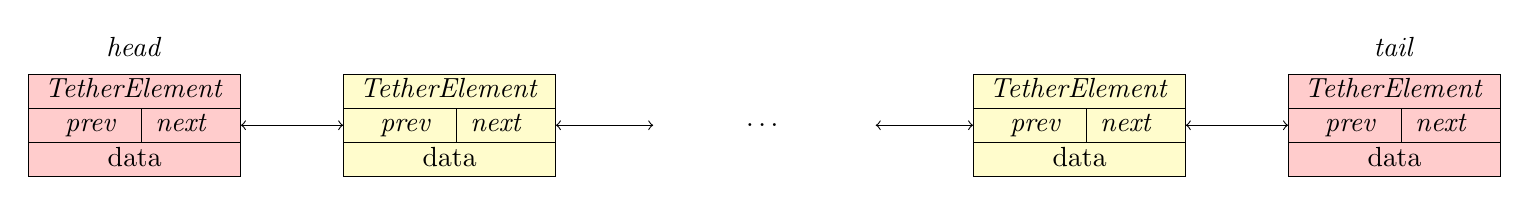
\begin{tikzpicture}
                \tikzset{TE/.style={draw, inner sep=0, outer sep=0, fill=yellow!20}}

                \node[TE, fill=red!20] (TE0) at (0,0) {\begin{tabular}{c} \textit{TetherElement} \\ \hline \hfill \textit{prev} \hfill \vline \hfill \textit{next} \hfill \\ \hline data \end{tabular}};

                \node[TE, fill=red!20] (TE4) at (16,0) {\begin{tabular}{c} \textit{TetherElement} \\ \hline \hfill \textit{prev} \hfill \vline \hfill \textit{next} \hfill \\ \hline data \end{tabular}};

                \foreach \i in {1,3} {
                    \node[TE] (TE\i) at (4*\i,0) {\begin{tabular}{c} \textit{TetherElement} \\ \hline \hfill \textit{prev} \hfill \vline \hfill \textit{next} \hfill \\ \hline data \end{tabular}};
                }
                \node[minimum width=80] (TE2) at (8,0) {\dots};
                \foreach \i in {0,1,2,3} {
                    \pgfmathtruncatemacro{\next}{\i +1}
                    \draw[<->] (TE\i) -- (TE\next);
                }

                \node (head) at (0,1) {\textit{head}};
                \node (tail) at (16,1) {\textit{tail}};
            \end{tikzpicture}
        }
        \caption{Liste doublement chainée}
        \label{fig:doubly_linked_list}
    \end{figure}

    \begin{figure}[!htb]
        \centering
        \resizebox{0.50\textwidth}{!}{
            \begin{tikzpicture}
                \begin{class}[text width=6cm]{Tether}{0,0}
                    \attribute{+ element\_mass : double}
                    \attribute{+ element\_volume : double}
                    \attribute{+ element\_length : double}
                    \attribute{+ position\_first : numpy.ndarray}
                    \attribute{+ position\_last : numpy.ndarray}
                    \attribute{+ elements : list of \textit{TetherElement}}
                \end{class}
            
                \begin{class}[text width=6cm]{TetherElement}{8.5,0}
                    \attribute{+ mass : double}
                    \attribute{+ volume : double}
                    \attribute{+ length : double}
                    \attribute{+ position : numpy.ndarray}
                    \attribute{+ velocity : numpy.ndarray}
                    \attribute{+ acceleration : numpy.ndarray}
                    \attribute{+ previous : TetherElement}
                    \attribute{+ next : TetherElement}
                    \attribute{+ K\_p : double}
                    \attribute{+ K\_d : double}
                    \attribute{+ K\_i : double}
                    \operation{+ F\_p(self) : numpy.ndarray}
                    \operation{+ F\_b(self) : numpy.ndarray}
                    \operation{+ F\_f(self) : numpy.ndarray}
                    \operation{+ Ft\_prev(self) : numpy.ndarray}
                    \operation{+ Ft\_next(self) : numpy.ndarray}
                \end{class}
            
                \aggregation{Tether}{}{~~~n}{TetherElement}
            \end{tikzpicture}
        }
        \caption{Diagramme de classe UML des classes \textit{Tether} et \textit{TetherElement}}
        \label{fig:uml_class}
    \end{figure}

\subsection{Suivi d'angles normalisés}
    Un problème avec la représentation numérique de l'orientation des solides est qu'elle est souvent normalisée, et les valeurs sont ainsi ramenées dans l'intervalle $[-\pi; \pi]$. On ne peut donc pas avoir l'orientation absolue, c'est à dire l'orientation d'un solide en prenant en compte les eventuels tours qu'il aurait pu faire sur lui-même.

    Pour résoudre ce problème, l'\textsc{Algorithme}~\ref{algo:suivi_angle} de suivi d'angles normalisés a été implémenté. Il prends en paramètres l'angle normalisé ainsi que l'angle précédemment calculé, et il retourne la valeur de l'angle absolu. L'idée de fournir l'angle précédent est de pouvoir retourner le nouvel angle qui se trouve dans le même quadrant et aussi de pouvoir suivre les sauts d'angles. Ainsi on peut suivre l'orientation absolue de solides en rotation dans l'espace, en ne fournissant que des orientations relatives ramenées dans l'intervalle $[-\pi; \pi]$, et en gardant en mémoire la précédente orientation calculée.
    
    \begin{algorithm}[!htb]
        \SetKwInOut{Input}{Entrées}
        \SetKwInOut{Output}{Sorties}
        \Entree{$angle\_normalise$, $angle\_absolu$}
        \Sortie{$angle\_absolu$}
        \Deb{
            $offset \leftarrow (angle\_absolu - angle\_normalise + \pi ) \pmod{2\pi}$ \\
            $angle\_absolu \leftarrow angle\_normalise + 2\pi \cdot offset$ \\
        }
        \Retour{$angle\_absolu$}

        \caption{Suivi d'angle} 
        \label{algo:suivi_angle}
    \end{algorithm}

    La \textsc{Figure}~\ref{fig:suivi_angle} présente les résultats de l'\textsc{Algorithme}~\ref{algo:suivi_angle} avec une angle variant dans l'intervalle $[-3\pi; 3\pi]$. On voit sur la première sous-figure l'angle réel et l'angle ramené dans l'intervalle $[-\pi; \pi]$ avec la présence de saut d'angles. Avec cette méthode, on est capable de suivre l'évolution de l'angle et de supprimer cess sauts afin de retrouver l'angle absolu visible dans la deuxième sous-figure et calculé uniquement à partir de la connaissance de l'angle normalisé.

    \begin{figure}[!htb]
        \centering
        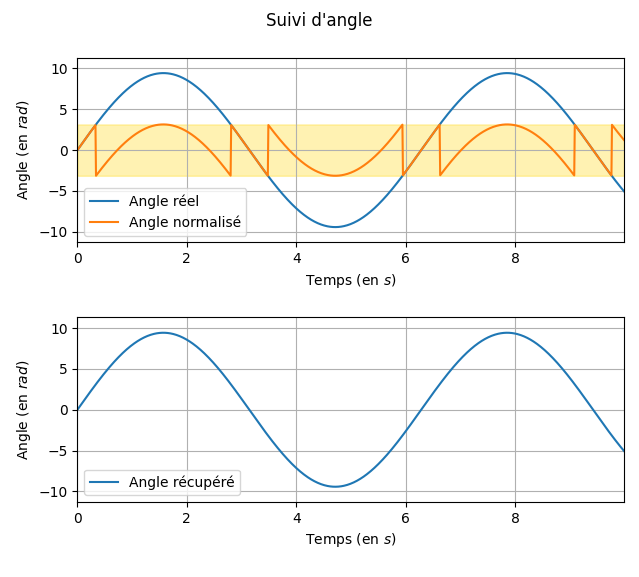
\includegraphics[width=0.5\textwidth]{suivi_angle.png}
        \caption{Suivi d'angle}
        \label{fig:suivi_angle}
    \end{figure}


\subsection{Resultats}
	

	\chapter{Simulation des robots}
	
	\section{Introduction}

		L'environnement dans lequel doivent évoluer les robots à été défini dans le \textsc{Chapitre}~\ref{chapitre:environnement}. Il est maintenant temps de simuler les \gls{ROV}s. Pour ce faire, nous allons devoir décrire les paramètres mécaniques des robots \gls{Argos} et \gls{Atoll}, ainsi que leurs capteurs et actionneurs à simuler.

	\section{Simulation des composants}
		En remarquant que les deux robots embarquent un certain nombre d'éléments communs, il est possible de definir et de simuler les différents composants dans \gls{Gazebo}, afin d'être par la suite chargés dans la simulation des deux robots. La \textsc{table}~\ref{table:components} présente les différents composants à simuler, s'ils nécéssitent l'utilisation d'un \gls{Plugin}, d'une \gls{HardwareInterface} et indique les dépendances entre les robots et ces composants.

		\begin{table}[!htb]
			\centering
			\begin{adjustbox}{max width=\textwidth}
				\begin{tabular}{|l|l|c|c|c|c|}
					\hline
					Composant & Description & \gls{Argos} & \gls{Atoll} & \gls{HardwareInterface} & \gls{Gazebo} \gls{Plugin} \\
					\hline
					\gls{Argos} Frame & Chassis d'\gls{Argos} & \cmark & \xmark & \xmark & \xmark \\
					\hline
					\gls{Atoll} Frame & Chassis d'\gls{Atoll} & \xmark & \cmark & \xmark & \xmark \\
					\hline
					Electronic Pod & Boîtier electronique & \cmark & \cmark & \xmark & \xmark \\
					\hline
					\gls{Latch} & Crochet de levage & \xmark & \cmark & \cmark & \cmark \\
					\hline
					\gls{Navcam} & Caméra de navigation & \cmark & \cmark & \xmark & \cmark \\
					\hline
					\gls{Obscam} & Caméra d'observation & \cmark & \cmark & \xmark & \cmark \\
					\hline
					Rovins & Centrale Inertielle & \cmark & \cmark & \xmark & \cmark \\
					\hline
					Spotlight & Lumières étanches & \cmark & \cmark  & \cmark & \cmark \\
					\hline
					SPE75 Thruster & Propulseur & \cmark & \cmark & \cmark & \cmark \\
					\hline
					SS309 Tilt & Nacelle pour caméra & \cmark & \cmark & \cmark & \cmark \\
					\hline
				\end{tabular}}
			\end{adjustbox}
			\caption{Composants à simuler}
			\label{table:components}
		\end{table}

		Chaque composant a ainsi un \gls{Package} de description qui lui est associe nommé suivant la convention de nommage \gls{ROS} : \textit{component\_description}. Ce package contient tout le code nécéssaire à la description du composant, c'est à dire un modèle \gls{Gazebo} permettant de simuler le composant dans le logiciel de simulation, un fichier de lancement qui s'occupe de lancer le composant dans le simulateur, les \gls{Mesh CAO}. Le code source d'un \gls{Plugin} permettant de décrire le comportement du capteur ou de l'actionneur associé au composant se trouve dans le package \textit{component\_model\_plugin}.

		Nous allons à présent détailler l'implémentation de certains composants qui ont un comportement intéressant à développer.

		\subsection{Latch}

			\subsubsection{Présentation}

				Le Latch est un composant propre au robot \gls{Atoll}. Ce crochet de levage permettant de transporter des structures sous-marines pouvant peser jusqu'à $1,5\ T$ est fabriqué par Forssea Robotics, et permet de positionner et de transporter des balises de positionnement acoustique sur les fonds marins.

			\subsubsection{Hardware Interface}


				
			\subsubsection{Model Plugin}
			
				Un \textit{Model Plugin} a été développé afin de décrire le comportement du \textit{Latch} dans \gls{Gazebo}. Il est basé sur la machine à états finis présenté en \textsc{Figure}~\ref{fig:latch_fsm} et crée un \gls{Joint} entre le \textit{Latch} et la structure à soulever de type encastrement. Les deux solides sont donc attachés l'un à l'autre jusqu'au moment où le signal de relâchement est envoyé au \textit{Latch} simulé, et le \gls{Joint} est alors supprimé.

				\begin{figure}[!htb]
					\centering
					\includegraphics[scale=0.8]{imgs/latch_fsm.pdf}
					\caption{Machine à états du \textit{Latch}}
					\label{fig:latch_fsm}
				\end{figure}

			\subsubsection{Résultats}

				On obtient alors le composant simulable dans l'environnement de simulation \gls{Gazebo}, comme on peut voir sur la \textsc{Figure}~\ref{fig:latch_gazebo}.

		\subsection{SS309 Tilt}

			\subsubsection{Présentation}

				Le \textit{SS309 Tilt} est un composant commercialisé par l'entreprise \textit{Sidus Solutions} et qui permet dans les \gls{ROV}s d'orienter l'\gls{Obscam}. Il est parfaitement étanche et comporte un jeu d'engrenages reliés à un moteur pas-à-pas pilotable en vitesse et en position. On demande ainsi au moteur de mettre l'axe à une certaine position, et l'axe se déplace avec une vitesse de rotation spécifiée.
			
			\subsubsection{Hardware Interface}

			\subsubsection{Model Plugin}

				Pour simuler cet aspect pilotable en vitesse de rotation et position, il faut passer par la simulation d'un moteur pas-à-pas. C'est un moteur un moteur composé de plusieurs bobinages créant ainsi plusieurs phases qui sont allumées succéssivement afin de réaliser une rotation de l'arbre moteur d'un certain incrément d'angle. Cet angle est défini par les caractéristiques du bobinage et n'est donc pas réglable. Il n'est pas non plus possible de piloter précisement la vitesse avec laquelle il se rend à cette position incrémentée. En revanche, il est tout à fait possible de connaître précisement la position du moteur, car l'arbre moteur ne peut prendre qu'un nombre fini d'angles, et il suffit donc de compter le nombre d'incréments commandés. Enfin, on peut commander la vitesse avec laquelle le moteur se rend à cette position, en allumant les phases à la vitesse désirée.

				Nous allons à présent distinguer la position réelle de l'arbre moteur, la position cible et la position commandée. La position réelle est la position de l'arbre moteur dans le simulateur. La position cible est un multiple de l'incrément d'angle à laquelle doit se rendre le moteur à l'instant actuel. La position commandée la position finale dans laquelle doit se retrouver l'arbre moteur et peut être une position réelle quelconque. Le moteur ne sera capable que de se rendre à la position multiple de la valeur de l'incrément d'angle la plus proche de la position commandée. La \textsc{Figure}~\ref{fig:tilt_position} reprends ces différentes notions. En commandant la vitesse à laquelle on incrémente la position cible, on contrôle l'axe en vitesse.

				\begin{figure}[!htb]
					\centering
					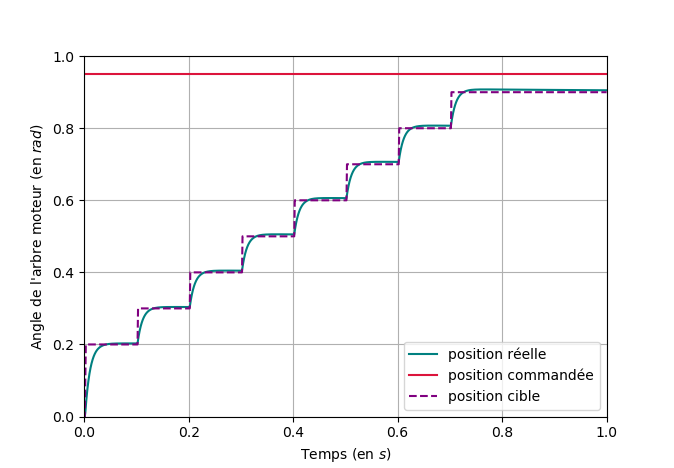
\includegraphics[width=0.6\textwidth]{imgs/stepper_motor.png}
					\caption{Simulation d'un moteur pas-à-pas}
					\label{fig:tilt_position}
				\end{figure}
				
				Pour ce qui est de l'implémentation de ce comportement dans \gls{Gazebo}, on crée un \textit{Thread} qui va s'executer en boucle avec une vitesse variable. Cette vitesse sera fonction de la vitesse de commande du \textit{Tilt} notée $\omega_c$. A chaque tour de boucle, on incrémente donc la position cible de la valeur de l'incrément $d\theta$ si la différence entre la position réelle et la position commandée est plus grande que ce même incrément, et on attends le temps $h$, avec :

				$$h = \frac{d\theta}{\omega_c}$$

				\begin{algorithm}[!htb]
					\caption{Algorithme de simulation d'un moteur pas-à-pas}
					\label{algo:stepper_motor}
					\begin{algorithmic}
						\WHILE {true}
							\STATE read $\theta_r$, $\omega_c$
							\IF {$|\theta_c - \theta_r| > d\theta$}
								\STATE $\theta_t \leftarrow \theta_t + d\theta$
							\ENDIF
							\STATE $h \leftarrow \frac{d\theta}{\omega_c}$
							\STATE sleep $h$
						\ENDWHILE
					\end{algorithmic}
				\end{algorithm}
				

	\section{Simulation d'Argos}

	\section{Simulation d'Atoll}

	\chapter{Resultats}
	
	\section{Introduction}

		Nous allons à présent tester le bon fonctionnement et analyser les résultats produits par le simulateur.
		
		Dans un premier temps, nous allons vérifier le respect des exigences présentées dans le \textsc{Chapitre}~\ref{chapitre:systeme}, ainsi que le comportement des robots et de l'environnement développés dans les \textsc{Chapitre}~\ref{chapitre:environnement} et \textsc{Chapitre}~\ref{chapitre:robots}.

		Ensuite, nous nous pencherons sur la comparaison du simulateur avec des expérimentations faites sur le terrain, afin de déterminer si les résultats de simulations sont proches du comportement réel des robots, et si ce système permet de réduire les temps de développements en en réduisant le nombre d'essais en conditions réelles à réaliser pour valider de nouvelles fonctionnalités.

	\section{Analyse du simulateur}

	\section{Comparaison avec les robots réels}

		Ecarts (statique/dynamique)


	\chapter{Gestion de projet}
	
	\section{Introduction}
		Ce rapport présente le travail effectué durant ce projet de fin d'études. Le format est particulier dans la mesure où j'ai réalisé la dernière année de ma formation en contrat de professionnalisation avec l'entreprise Forssea Robotics. J'ai donc pu travailler pendant un an avec eux, en commencant par 6 mois durant lesquels j'ai fini ma formation au sein de l'\gls{ENSTAB}, puis 6 mois durant lesquels j'ai pu travailler à temps plein sur mon projet de fin d'études. Cela présente l'avantage d'avoir à sa charge la gestion d'un projet plus complet, puisque le temps le permet, comparé à un projet de fin d'étude classique dans lequel il est souvent confié au stagiaire la réalisation d'une tâche d'un projet.

	\section{Méthodologie}
		Les \textit{Methodes Agiles} forment un ensemble de méthodes facilitant la gestion de projet, qui sont particulièrement adaptées au monde du développement logiciel. Il permet de réaliser une plannification adaptative, un développement évolutif et une amélioration continue du produit. Elles s'opposent aux méthodes plus traditionnelles, comme les méthodes séquentielles de type \textit{Cycle en V}, qui s'adaptent très mal à ce type de produit. Elles permettent aussi d'avoir un produit utilisable par le client, avec des fonctionnalités qui évoluent au cours du développement.

		La \textit{Methode Scrum} est un cadre hérité de la \textit{Méthode Agile} permettant lui aussi de gérer le développement d'un produit. Il se distingue des \textit{Méthodes Agiles} dans la mesure où ce n'est pas seulement un ensemble de concepts, mais plutôt ici un ensemble de règles à suivre pour gérer correctement un projet. La \textit{Méthode Scrum} nécéssite la désignation de :

		\begin{itemize}
			\item Un \textit{Scrum Master} : garant de l'application de la \textit{Méthode Scrum},
			\item Un \textit{Product Owner} : garant des attentes du client au sein du projet,
			\item Une équipe de développement : réalisant le produit.
		\end{itemize}

		Les temps forts de la \textit{Méthode Scrum} sont :

		\begin{itemize}
			\item La plannification de \textit{sprint} : réunion durant laquelle les nouvelles fonctionnalités à ajouter au produit sont séléctionnées en accord avec le \textit{Product Owner},
			\item La revue de \textit{sprint} : réunion se déroulant en général après le sprint et durant laquelle les nouvelles foncitonnalités implémentées durant le \textit{sprint} sont présentées au \textit{Product Owner} et au client, et le prochain sprint est préparé,
			\item La retrospective de \textit{sprint} : réunion dans laquelle l'équipe analyse sa propre gestion de projet en terme d'efficacité, de qualité, de productivité,
			\item La mêlée quotidienne : réunion dans laquelle l'équipe de développement expose ce qu'elle a réalisé, ce qu'elle va réaliser et les problèmes qui ont été rencontrés depuis la dernière mêlée.
		\end{itemize}
	
		Lors du développement du simulateur réalisé pendant ce projet de fin d'étude, une \textit{Méthode Scrum} a été utilisée, dans la mesure où c'est la méthode qui est utilisée par le reste de l'entreprise. On peut cependant la qualifier de légère, car les \textit{sprints} n'étaient pas très formalisés, d'abord car j'étais le seul développeur en charge de ce projet de simulation. Le choix des nouvelles fonctionnalités à prendre en compte était décidé lors d'une réunion hebdomadaire servant de point d'avancement du produit. Les réunions quotidiennes étaient cependant bien présente, et elle permettaient d'avoir à l'esprit ce que les autres développeurs étaient en train de faire. En outre la start-up est divisée en trois pôles : Robotique, Vision et Mécanique. Les réunions quotidiennes étaient séparées par pôles afin d'être plus efficace, mais une réunion mensuelle venait synchroniser les différentes équipes afin de définir les objectifs réalisés et à venir pour l'entreprise.

	\section{Outil de gestion de projet}

		Un outil intéressant pour appliquer la \textit{Méthode Scrum} est le service \textit{Jira} d'\textit{atlassian}\footnote{\url{https://www.atlassian.com/fr/software/jira}}. C'est un outil développé pour appliquer ces méthodes de gestion de projet en équipe, avec une intégration des différents concepts et des différentes règles inhérentes à ces procédés. Il permet de facilement planifier le projet, le suivre, mais aussi de livrer facilement et de créer des rapports de fonctionnalités, des notes de versions et autres notices utiles pour l'utilisateur final.

		Le service \textit{Github}\footnote{\url{https://github.com/}} permet lui de versionner et de travailler facilement en collaboration sur du code. Basé sur le logiciel de versionning \textit{Git}\footnote{\url{https://git-scm.com/}}, ce service propose la possibilité de créer des organisaitons, et donc d'avoir une entité possédant tout le code développé pour le produit.
		
		Ces deux outils sont parfaitement intégrés ensemble. En effet, le suivi d'implémentation est automatique entre \textit{Jira} et \textit{Github}, et dès qu'une nouvelle fonctionnalité est ajoutée, elle est automatiquement classée comme implémentée. Un système de tests unitaires permettent aussi de tester en intégration le code implémenté, afin d'être sûr que le code est foncitonnel.

	\chapter{Conclusion}
	\label{chapitre:conclusion}
	
	\section{Conclusion technique}

		La réalisation de ce simulateur est un point très important dans le domaine du développement robotique. Je suis conscient des gains apportés par un tel système en terme de coûts de développements, car les essais en robotique restent très onéreux, la puissance de calculs de nos ordinateurs sont aujourd'hui largement suffisantes, et les logiciels de simulations de plus en plus complets et puissants. 
		
		Un exemple marquant est que durant mon projet de fin d'études, une semaine d'essais prévue n'a quasiment servie à rien, car le bateau censé être utilisé pour la campagne d'essais n'a pas pu quitter le port à cause d'un problème météorologique. Cela a nécéssairement mobilisé du matériel et des hommes pour tester des fonctionnalités qui auraient pu être testée en simulation dans un premier temps, avant de réaliser une campagne d'essais finale permettant de valider la nouvelle version complète du robot.
	
	\section{Conclusion du projet}

		Ce simulateur a été réalisé durant un contrat de professionnalisation avec \textsc{Forssea Robotics} et dans la continuité de mon stage de deuxième année réalisé aussi sur des aspect de simulation en développement robotique sur \gls{Gazebo} dans la jeune pousse \textsc{Exxact Robotics}. J'ai donc pu me spécialiser cette dernière année dans la simulation robotique et notamment sur l'utilisation du simulateur \gls{Gazebo} qui est très permissif et dans lequel j'ai pu beaucoup apprendre.

		En terme de gestion de projets, il a été très intéressant d'avoir à ma charge la gestion de l'intégralité du projet simulation. Je trouve que c'est une bonne introduction à mon futur parcours professionnel, et l'encadrement de mon maître de stage m'a permis de mener à bien ce projet.

		La conception de ce système m'a amené à formaliser beaucoup d'aspects du simulateur, et le côté start-up de \textsc{Forssea Robotics} fait que les projets sont axés recherche et développement. Cela a éveillé en moi un attrait pour la recherche et m'incite à continuer mes études dans le monde de la recherche par la réalisation d'une thèse à la suite de ce projet de fin d'études.
	
	\appendix
	\cleardoublepage
	\pagenumbering{roman}
	\chapter{Annexes}
\label{annexe:gantt}

	Demo équation de la chainette

	\clearpage

	\begin{figure}[H]
		\centering
		\rotatebox{90}{
			\includegraphics[width=21cm]{./gantt/gantt.pdf}
		}
        \label{fig:gantt}
        \caption{Diagramme de Gantt prévisionnel du projet}
	\end{figure}

	\clearpage

	\begin{figure}[H]
		\centering
		\rotatebox{90}{
			\includegraphics[width=21cm]{./gantt/gantt.pdf}
		}
        \label{fig:gantt}
        \caption{Diagramme de Gantt final du projet}
	\end{figure}

	\clearpage
	\phantomsection
	\chapter{Liste des Figures}
	\makeatletter
	\@starttoc{lof}% Print List of Figures
	\makeatother


	\clearpage
	\phantomsection
	\chapter{Liste des tableaux}
	\makeatletter
	\@starttoc{lot}% Print List of Tables
	\makeatother

	\clearpage
	\phantomsection
	\label{sec:index}
	\addcontentsline{toc}{chapter}{Index}
	\printindex

	\printglossaries


	\clearpage
	\phantomsection
	\addcontentsline{toc}{chapter}{Bibliographie}

	\bibliography{bib/sea,bib/intro,bib/software.bib}
	\bibliographystyle{ieeetr}

\end{document}
